% From Skoltech's requirements:
%
% > The main part includes:
% > - A description of the history and background literature on the subject
% > - Statement of research problem
% > - Statement of methodology
% >     - Design, data collection, analysis, interpretation
% > - Results
% > - Discussion of innovation and research findings
% > 
% > Justification of reseach relevance is mandatory.


\chapter{Premises} \label{chap:premises}

\section{Emergence of hyperbolic deep learning} \label{sec:history}

In
2015-2018~\cite{spaceTimeEmbeddings,nickelKiela17,embeddings2018dhingra,wilson2018gradient}
it came to attention of deep learning community, that for a
Euclidean space of fixed dimension, \( \mathbb{R}^n \) with usual distance
function, there are graphs which cannot be isometrically embedded in it, and
that any graph could be isometrically embedded in a Hyperbolic space.
\citet{spaceTimeEmbeddings} demonstrate many setups possible in Hyperbolic
spaces but not flat spaces.
Sarkar~\cite{sarkar} gives a combinatorial algorithm for approximately
isometric embedding of a tree. This has inspired a number of works using
hyperbolic representations for graph-like data, for instance in language models

\subsection*{NPC spaces}

First we need to define what a ``hyperbolic space'' is. First of all, a
hyperbolic space is a metric space -- i.e. it is a set of points and it has a
distance function. However its distance function is very special.
Specifically, a metric space is called hyperbolic if it has constant negative
curvature. A simpler related concept of non-positive curvature (and, similarly,
upper-bounded and lower-bounded curvature) can be described in terms of
compairson triangles, see~\autoref{fig:npcSpaces}. In your metric space,
consider three points $p, q, r$ in a small neighbourhood.  Connected by
geodesics, they form a triangle with sides $|pq|$, $|qr|$, and $|rp|$ ($|xy|$
for distance between $x$ and $y$).  One could construct a unique Euclidean
triangle with same sides. Next, one could
measure how distance from base point $p$ to the midpoint $\gamma_t$ between $q$
and $r$ compares to its Euclidean counterpart. In hyperbolic space the midpoint
will appear closer than Euclidean prediction suggests, and on a
(positively-curved) sphere the opposite inequality is true. One could also
measure sums of angles -- in hyperbolic space they are strictly less than
$\pi$, or how volume of a ball grows with its radius -- in hyperbolic space it
is exponential. An important observation is that spaces of different constant
curvature cannot be isometric

We treat the notion of ``curvature'' in more detail in
Appendix~``\nameref{chap:manifolds}'' and specifically~\autoref{sec:curvature}.
Section ``\nameref{sec:poincareBall}'' in the
Appendix~``\nameref{chap:hyperbolics}'' introduces a concrete example of a
hyperbolic space.

\begin{figure}[ht]\center
    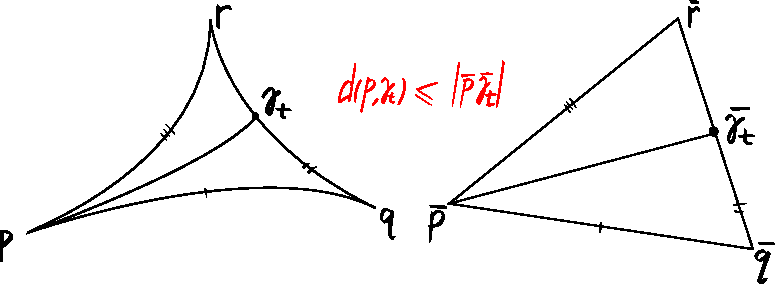
\includegraphics[width=.9\textwidth]{art/npc-comparison-triangle.pdf}
    \caption{Triangles in non-positively curved spaces versus flat (Euclidean) spaces.
    The intermediate point \( \gamma_t \) appears closer to \( p \)
    than a prediction based on Euclidean comparison suggests}
    \label{fig:npcSpaces}
\end{figure}

\subsection*{Curvature in metric graphs}

Consider a graph that consists of vertices connected by edges. Such a graph is
naturally
a metric space -- its points are the nodes of the graph, and distances are
measured in smallest number of edges on has to travel to get from one node to
another.  Such distances can behave very wildly, compared to
distances in Euclidean
space. For instance, you could have any number of points that are
simulataneosuly nearest neighbours of each other (consider the fully-connected
graph \( K_n \)), whereas in a two-dimensional Euclidean
plane~\cite{howManyNeighbours} the best you can do is three points allocated in
an equilateral triangle. This has immediate implications if you were to define
the notion of ``similarity'' of objects (images or words) in terms of distance
between their embeddings.  For instance, we could say that objects are
``similar'' if the ``distance'' between them is no more than \( 1 \) (an
arbitrarily chosen threshold).  That's a binary relation, and with
graph-distances such relation could well be non-transitive (``$A$ similar to
$B$ and $B$ similar to $C$ does not entail $A$ similar to $C$''). This is easily
seen
in a tree of constant branching factor: the sibling nodes are both ``similar''
to their common immediate parent, but not to each other. Ball volumes and
sphere areas also grow exponentially, see~\autoref{fig:binaryTreeCircumference}.
For a ``branchy'' enough tree, such relationships simply cannot be modeled by
distances between Euclidean embeddings (of pre-defined dimension).

This observation -- that many trees and graphs have strictly negative curvature --
implies one couldn't even hope, in general, to isometrically embed a graph in \(
\mathbb{R}^n \).

\begin{figure}[ht]\center
    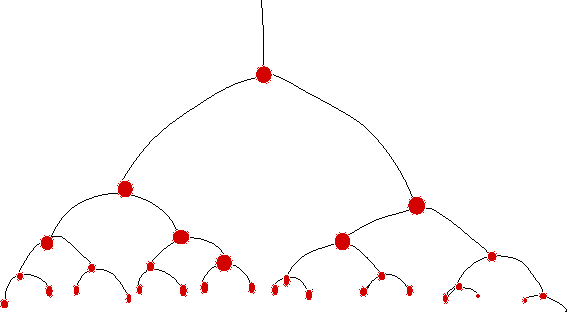
\includegraphics[width=.9\textwidth]{art/binary-tree-circumference-min.pdf}
    \caption{A full binary tree has \( 2^n \) nodes on \( n \)'th level, i.e.
    circumference of a sphere in this metric space grows exponentially with the
    radius. The volume of a ``ball'' of radius \( n \) centered at root would
    also be exponential, \( 2^{n+1} - 1 \).}
    \label{fig:binaryTreeCircumference}
\end{figure}

\subsection*{Hyperbolic Neural Networks}

\citet{ganeaHNNs} introduce hyperbolic neural layers which operate on
hyperbolic embeddings and can be arbitrarily stacked into deep networks.
For example, they construct a Gated Recurrent Unit with hyperbolic hidden
state.
To save space, we cover this subject in more detail (including references) in
the appendix~\nameref{chap:hyperbolics}. \nameref{chap:manifolds} may be a
prerequisite for that section.

\subsection*{Hyperbolic Image Embeddings}

\citet{khrulkov} endeavour to explore ``hidden hierarchies'' of classes of
objects in image datasets, like \texttt{MiniImageNet}. Specifically, in the
revised pre-print they measure \( \delta \)-hyperbolicity of Euclidean distance
between embeddings of images to reason about ``hierarchicity'' of a dataset.
They then improve off-the-shelf CNNs by appending exponential map layer on top
of them and use hyperbolic distances between embeddings for the final
decision rule (as in~\citet{snell2017protonet}).

\subsection{Convolutions for ``hyperbolic arrays''} \label{sec:hconv}

\begin{figure}[ht]\center
\begin{tikzpicture}
\node at (0,0) {
    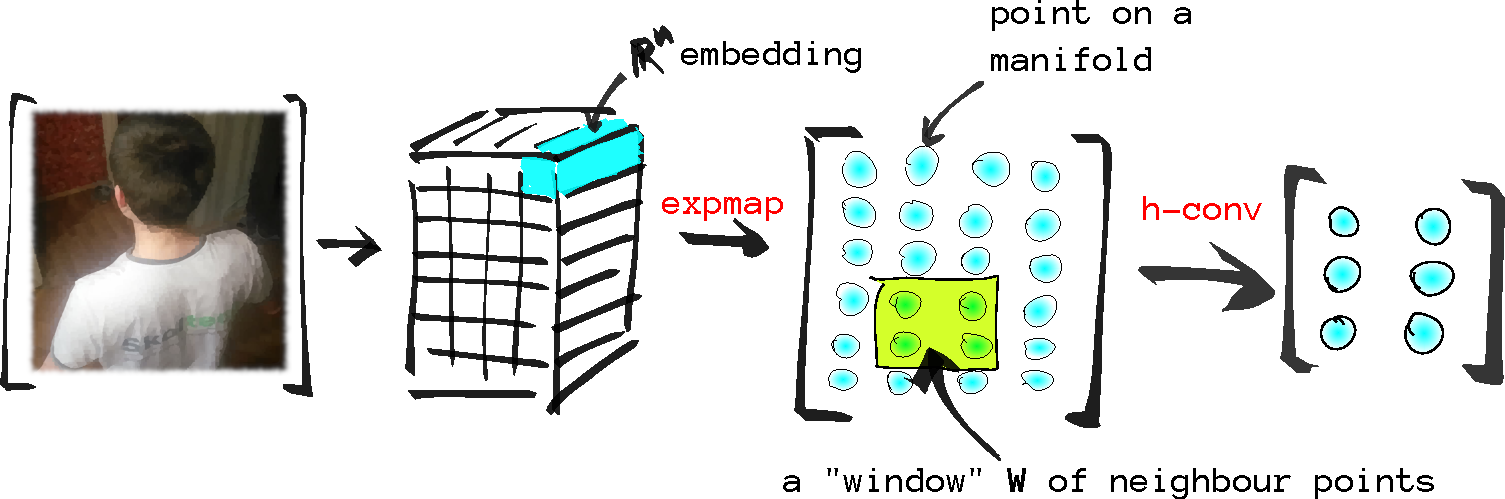
\includegraphics[width=.9\textwidth]{art/image-convolutions-2019.pdf}
};
\end{tikzpicture}
\caption{A visualization of ``hyperbolic'' CNN for representation learning}
\end{figure}

In \emph{very} short: we (Max Kochurov, Rasoul Karimov, Maria Taktasheva,
Cyrill Mazur, Serge Kozlukov) attempt to construct ``convolutional'' layers
which ``consume'' (multidimensional) arrays of \emph{points on manifolds} (each
point interpreted as a ``descriptor of a pixel'') -- ``hyperbolic arrays''. Our
idea is that hyperbolic space is a continuous analogue of a tree and our
convolutional operation resembles a ``decisison rule for walking down the
tree'', choosing new directions based on descriptors of neighbour pixels. We
also generalize Batch Normalization to such setting by appealing to the notion
of variance and (variance-minimizing) barycenter of a measure in a metric
space. Experiments showed these models to quickly overfit with very small number
of parameters (\( 100 \)K parameters are enough to overfit on CIFAR10),
however we couldn't find a way to regularise the model to improve generalization
ability. For this reason, we omit detailed description of these results here.
The general idea, however, is relevant to the rest of the work. A number
of questions have been left open: whether and which non-linearities are needed
in hyperbolic networks, how to transport filters between points, how to even
justify the framework?

Later, \citet{bouza2020mvc} considered a somewhat similar model for
``convolutions', and \citet{chakraborty2020manifoldnorm} proposed a similar
normalization layer.

\section{Equivariant CNNs} \label{sec:equivariant}

A parallel line of geometric methods' development relates to the idea of
equivariance. The most succesful idea in deep learning is arguably that of
convolutional networks. Convolutional neural networks (CNNs) convolve
input signals with a number of learned filters, each filter capturing
its own pattern. To be specific, a convolution of a function \( f: \mathbb{R}^n
\to \mathbb{R} \) and a filter \( h: \mathbb{R}^n \to \mathbb{R} \) is the
function~\cite{feichtingerFAHA}
\[ f*h = x \mapsto \int_{\mathbb{R}^n} f(y + 0) h(x-y)
\operatorname{d\lambda} y. \]
In case of discrete signals, such as images, this
integral reduces to a finite sum over pixels. An important thing to notice
about this operation, is that it commutes with translations:
\[ (T_a f) * h = f * (T_{-a} h) = T_a (f * h), \]
where \( T_a f = x \mapsto f(x + a) \).

This is exactly what makes the pattern-matching behaviour of CNNs possible: the
filter captures the pattern no matter how the input image has been translated
(i.e. regardless of where the matching object is located). \citet{s2cnn} note
however that such CNNs still have to learn separate filters for rotated
versions of the same object. Further, they consider the problem of spherical
input signals (think heatmaps over the surface of the earth) which possess
rotational and not translational symmetries. However, harmonic analysis can be
performed on groups different from translations, the convolution
formula becoming
\[
(f * h)(x) = \int_G f(g e) h(g^{-1}x) \operatorname{d}g,
\]
for \( f \) and \( h \) of type \( M\to N \), and \( G \) a group acting on
\( N \).

\citet{s2cnn,cohen2018general,e2cnn} build on this idea and propose
convolutional layers equivariant with respect to different groups of
transformations.

For a more detailed treatment of (non-Euclidean) Harmonic analysis one could
refer
to~\citet{axlerHarmonic,
elliott2019generalized,
explorationsHarmonic,
benedettoHarmonic,
stollharmonic,
terrasHarmonicSymmetric,
terrasHarmonicSymmetric2,
fourierS2},
while the bridge to the classic Harmonic analysis could be found in the already
metnioned~\cite{feichtingerFAHA}.
\citet{eyeRotations,zhou2019glosh,scnnNiessner} are another kind of appearances
of Harmonic analysis concepts.

\section{Graph convolutions}

One more direction for geometric methods is neural networks operating on graphs.
We refer the Reader to~\citet{kipf}.

Graph-convolutional methods are also being used for 3D data. The Reader might
take a look at~\citet{edgeconv} which is particularly relevant to this thesis.

\section{Geoopt} \label{sec:geoopt}

This thesis is closely related to the geoopt~\cite{geoopt} package, a joint
effort of Max Kochurov, Rasoul Karimov, and your narrator.
Geoopt is Python package for Riemannian optimization in \texttt{PyTorch}.
More background on Riemannian optimization is in the Appendix~\nameref{chap:manifolds}.
Starting this development, the authors hadn't much familiarity with
differential geometry, nor with optimization on manifolds in particular. One of
the consequences is that we simply couldn't have been aware of what use-cases
are important, thus in spite of rather hot discussions, the final API has
significant flaws.

A very short overview of the current design: \texttt{geoopt.Manifold} base
class describes a methodset expected by \texttt{geoopt.optim} optimizers (which
are compatible with \texttt{torch.optim}); this methodset includes
\texttt{retr}action, vector \texttt{transp}ort, \texttt{inner} product, and its
inverse, \texttt{egrad2rgrad} (see \nameref{sec:metricMfds} on how inner
product is related to conversion between ``Euclidean and Riemannian
gradients''); specific implementations of \texttt{Manifold}
can substitute different versions of e.g. retractions, providing different
levels of precision; points and tangent vectors are always represented by
coordinates in the (assumed) ambient space. In case of \texttt{PoincareBall}
(\autoref{sec:poincareBall}),
this coincides with the natural global chart and its chart-induced basis vector
fields (defined in appendices, \nameref{sec:chartInducedBasis}). Such
consistency is only possible because of negative curvature of
Hyperbolic space and conformality of Poincar\'e Ball.
On a sphere one could neither allocate a non-vanishing smooth
vector field, nor expect unique geodesics to exist between all points, nor measures to
have unique barycentres.

To be precise, the numbers that Geoopt stores to
represent a tangent vector are actually coordinates of the push-forward of that
vector under assumed embedding into ambient vector space. Restricting ourselves
to such representations wasn't an easy and immediate decision, but at the time
we couldn't find useful use-cases for introducing e.g. local charts.

\subsection{Current limitations of geoopt} \label{sec:geooptTodo}

``...since brevity is soul of wit, and tediousness the limbs and outward
flourishes, I will be brief'':
\begin{itemize}
\item An important use-case for introducing local charts to geoopt is tiling-based
parameterizations of Hyperbolic space, as in~\citet{yaSaTilingBased}
\item As~\citet{trivializations} suggests, we should further our discussion of
``manifold versus methodset-for-optimization'' interface, as in addition to
retraction-based optimization, we may be interested in Riemannian and Lie
exponentials with tangent-space parameterization and adaptive schemes.
\item Currently, dimension of manifold is not part of the \texttt{Manifold}
type nor of \texttt{manifold} object, which limits both type-checking and
inference opportunities.
\item Finally, geoopt is implemented in PyTorch. This implies inconvenient
    bounds to PyTorch's hierarchy of classes, consequent type mismatches and
        type erasures.  A functional style rewrite in JAX~\cite{jax2018github} would allow less
        \emph{flawed} design, higher order differentiation, as well as more
        consistent language (authors of JAX follow Spivak's ``Introduction to
        Differential Geometry''~\cite{spivak1970comprehensive} and
        SICP~\cite{abelson1996structure} authors' ``Functional Differential
        Geometry''~\cite{sussman2013functional}).
\end{itemize}

\section{Aims and research statement} \label{sec:statement}

To summarize the above, we believe that in problems involving ``complex
hierarchies'', the performance of any off-the-shelf model can be improved by
accounting for curvature in the right way. In previous experiments, however, we
weren't able to figure out what this ``right way'' is. We observe parallels
with Harmonic analysis on manifolds and with works of Cohen and Welling on
exploiting symmetries in data. Our goal is to incorporate insights from these
related methods into our models in order to possibly fix their failures.
For simplicity, we evaluate our ideas on image classification and pointcloud
classification.  The results are reported in chapter~\nameref{chap:conclusion}.
